% Latex template for submission to the 16th International Meeting on Fully 3D Image Reconstruction 
% in Radiology and Nuclear Medicine (Fully3D 2021)
%
% Author: G.Schramm
% Date:   Oct 2020
%
% In case you encouter problems, you can raise a github issue here:
% https://github.com/gschramm/fully3d_2021_templates/issues
%
% 
% To build this document, we recommend to use latexmk via:
% ```latexmk -pdf fully3d_template.tex```
% Building in the online editor overleaf also works.

\documentclass[11pt,twocolumn,twoside]{article}
\usepackage{fully3d}

%%%%%% add your extra packages here (if needed)                                       %%%%%
%%%%%% before, have a look which packages are already imported by the fully3d package %%%%%

\usepackage{amssymb}
\usepackage{algorithmicx}
\usepackage{algpseudocode}
\usepackage{grffile}
\usepackage{caption}
\usepackage{subcaption}
\usepackage{lipsum}

%\usepackage{sfmath}
%\renewcommand\familydefault{\sfdefault}
%\definecolor{light-gray}{RGB}{242,242,242}
%\pagecolor{light-gray}

%\newtheorem{rem}{Remark}

% define float env for algorithm
\usepackage{float}
\floatstyle{ruled}
\newfloat{algorithm}{h}{loa}
\floatname{algorithm}{Algorithm}

%%%%% add your bibtex file that contains the bibtex entries here %%%%%
%%%%% please include DOIs in the bibtex entries if possible      %%%%%
%\addbibresource{fully3d_2021.bib}

% custom definitions
\DeclareMathOperator{\proj}{proj}
\DeclareMathOperator{\prox}{prox}
\DeclareMathOperator*{\argmin}{arg\,min}

\begin{document}


%-------------------------------------------------------------------------------------------
%%%%% add your title here %%%%%
\title{Fast and memory-efficient list-mode reconstruction of sparse TOF PET data with non-smooth convex priors}

%%%%% add authors and affiliations here %%%%%
\author[1]{Georg~Schramm}
\author[2]{Martin~Holler}

\affil[1]{Department of Imaging and Pathology, Division of Nuclear Medicine,
          KU Leuven, Belgium}

\affil[2]{Institute of Mathematics and Scientific Computing, 
          University of Graz, Austria}

%%%%% don't change these 2 lines %%%%%
\maketitle
\thispagestyle{fancy}



%-------------------------------------------------------------------------------------------
%%%%% add your summary (abstract) here               %%%%%%
%%%%% use footnotesize for this section              %%%%%%
%%%%% please stick to the customabstract environment %%%%%% 


\begin{customabstract}
foo bar
\end{customabstract}

\section{Introduction}

\lipsum[2-4]

%-------------------------------------------------------------------------------------------
%%%%% main text %%%%%    
\begin{equation}
\argmin _{x\geq 0} \sum_j (Px)_j -  d_j \log \left( (Px)_ j + s_j \right) + R (K x),
\end{equation}

%-----------------------------------------------------------------------------
\begin{algorithm}[t]
\begin{algorithmic}[1]
\small
\State \textbf{Initialize} $x(=0),y(=0),(w=0)$, $(S_i)_i,T,(p_i)_i$,
\State $\overline{z} = z = P^T y + K^T w$
\Repeat
	\State $x = \proj_{\geq 0} (x - T \overline{z})$
	\State Select $i \in \{ 1,\ldots,n+1\} $ randomly according to $(p_i)_i$
  \If{$i \leq n$}
	\State $y_i^+ \gets \prox_{D_i^*}^{S_i} ( y_i + S_i  ( P_i x + s_i))$
	\State $\delta z \gets P_i^T (y_i^+ - y_i)$
	\State $y_i \gets y_i^+$
  \Else
	\State $w^+ \gets \prox_{R^*}^{S_i} ( w + S_i  K x)$
	\State $\delta z \gets K^T (w^+ - w)$
	\State $w \gets w^+$
  \EndIf
	\State $z \gets z + \delta z$
	\State $\overline{z} \gets  z + (\delta z/p_i)$
\Until{stopping criterion fulfilled}
\State \Return{$x$}
%\EndFunction
\end{algorithmic}
\caption{SPDHG for PET reconstruction}
\label{alg:spdhg}
\end{algorithm}

%-----------------------------------------------------------------------------
\begin{algorithm}[t]
\begin{algorithmic}[1]
\small
\State \textbf{Input} event list $N$
\State \textbf{Calculate} event counts $\mu_e$ for each e in $N$ (see text)
\State \textbf{Split} event list $N$ into $m$ sublists $N_i$
\State \textbf{Initialize} $x,w,(S_i)_i,T,(p_i)_i$
\State \textbf{Preprocessing} $\overline{z} = z = P^T y + K^T w$ (see text)
\State \textbf{Initialize} $m$ sub lists $l_{N_i}$ with 0s
\Repeat
	\State $x = \proj_{\geq 0} (x - T \overline{z})$
	\State Select $i \in \{1,\ldots,m+1\}$ randomly accord. to $(p_i)_i$
  \If{$i \leq m$}
	  \State $l_{N_i}^+ \gets \prox_{D^*}^{S_i} \left( l_{N_i} + S_i \left(P^{LM}_{N_i} x + s_{N_i} \right) \right)$
	  \State $\delta z \gets {P^{LM}_{N_i}}^T \left(\frac{l_{N_i}^+ - l_{N_i}}{\mu_{N_i}}\right)$
	  \State $l_{N_i} \gets l_{N_i}^+$
  \Else
	  \State $w^+ \gets \prox_{R^*}^{S_i} \left( w + S_i K x \right)$
	  \State $\delta z \gets K^T \left(w^+ - w\right)$
	  \State $w \gets w^+$
  \EndIf
	\State $z \gets z + \delta z$
	\State $\overline{z} \gets  z + (\delta z/p_i)$
\Until{stopping criterion fulfilled}
\State \Return{$x$}
%\EndFunction
\end{algorithmic}
\caption{LM-SPDHG for PET reconstruction}
\label{alg:lmspdhg}
\end{algorithm}



%-----------------------------------------------------------------------------

\section{Results}

\begin{figure*}
  \centering
    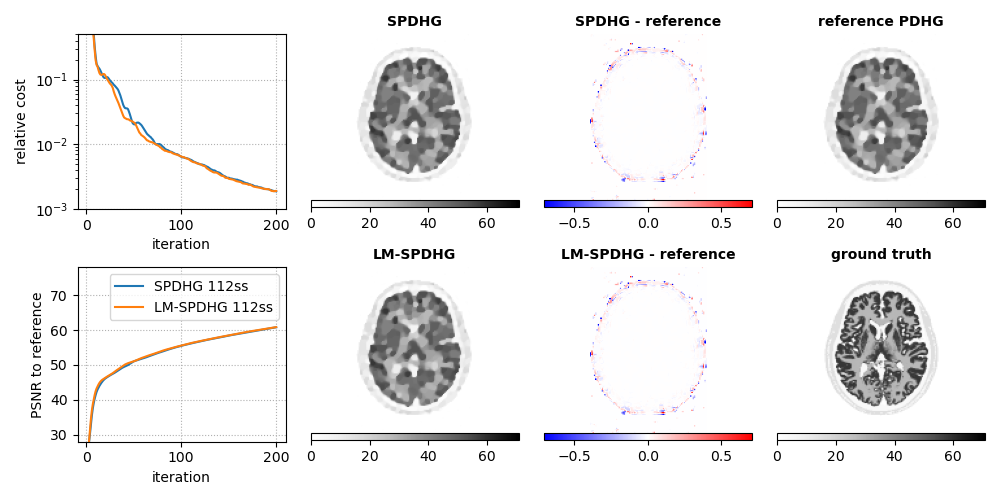
\includegraphics[width=1.0\textwidth]{./figs/brain2d_counts_1.0E+06_seed_1_beta_3.0E-02_prior_TV_niter_ref_20000_fwhm_4.5_4.5_niter_200.png}
    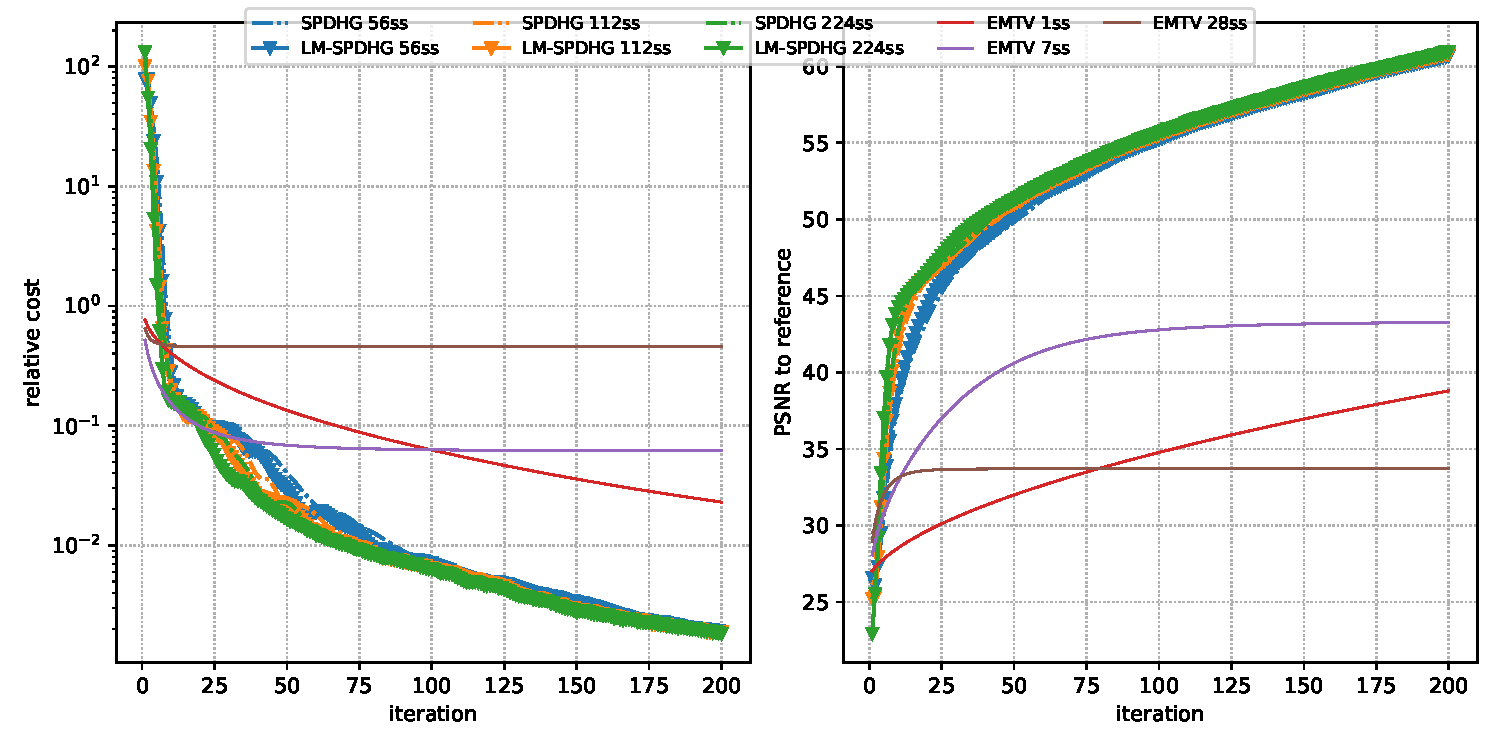
\includegraphics[width=0.8\textwidth]{./figs/brain2d_counts_1.0E+06_seed_1_beta_3.0E-02_prior_TV_niter_ref_20000_fwhm_4.5_4.5_niter_200_metrics.pdf}
  \caption{$1\cdot10^6$ counts, TV, $\beta = 0.03$}
  \label{fig:metrics}
\end{figure*}

\begin{figure*}
  \centering
    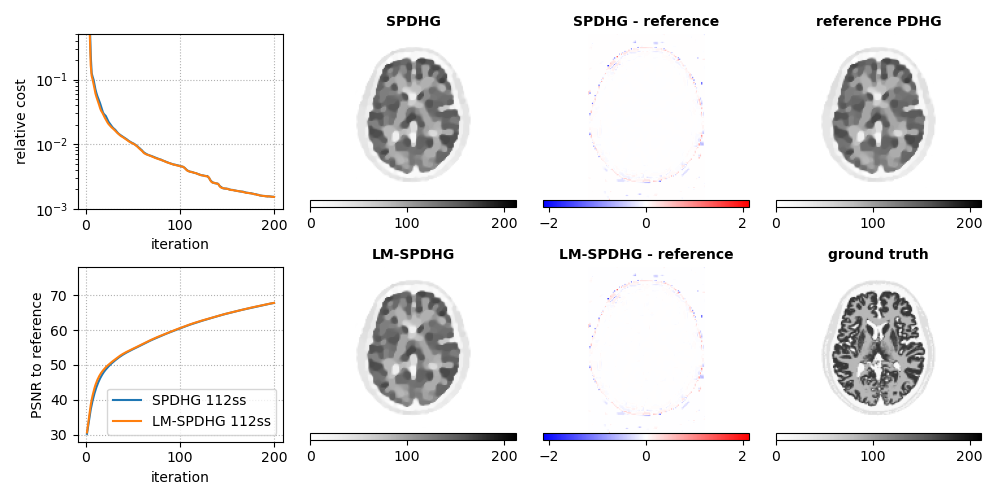
\includegraphics[width=1.0\textwidth]{./figs/brain2d_counts_3.0E+06_seed_1_beta_3.0E-02_prior_TV_niter_ref_20000_fwhm_4.5_4.5_niter_200.png}
    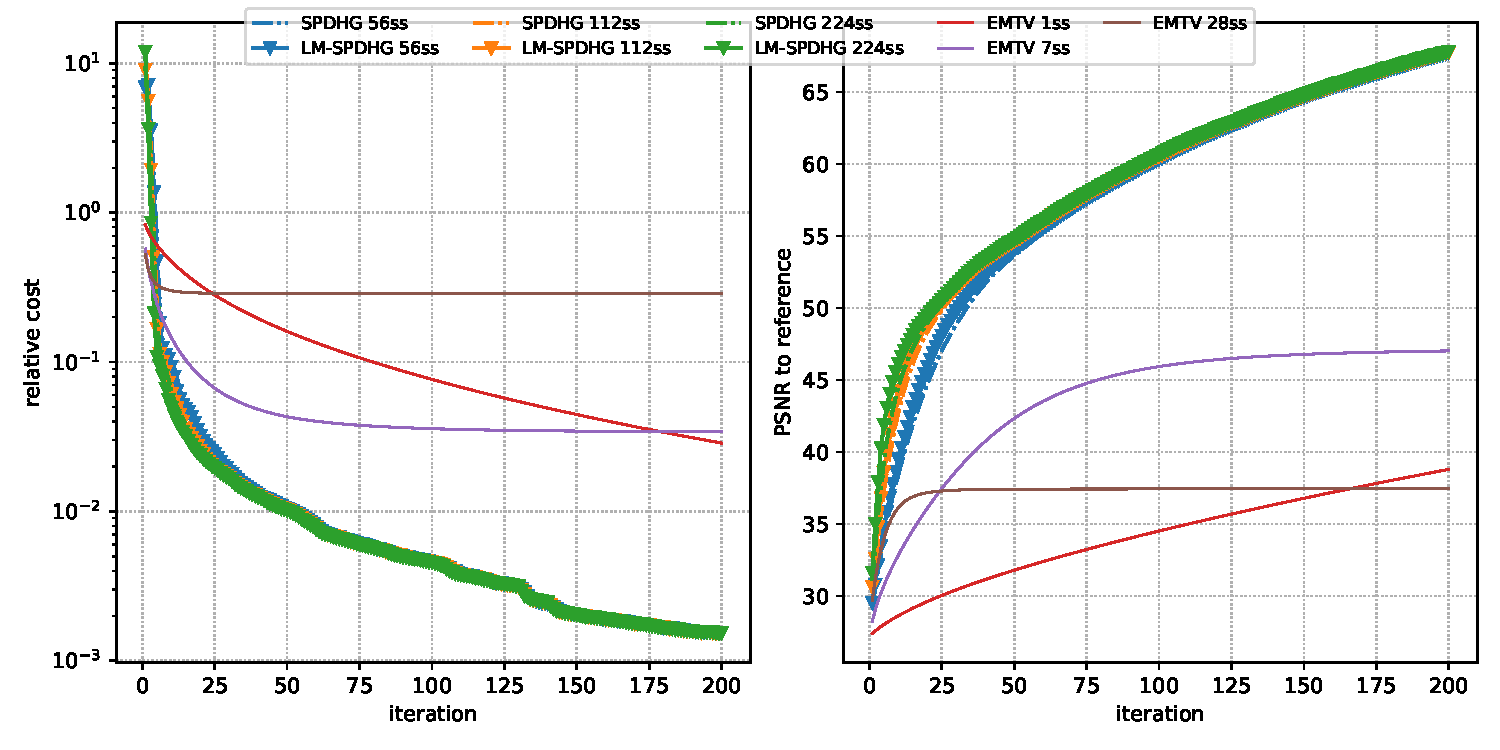
\includegraphics[width=0.8\textwidth]{./figs/brain2d_counts_3.0E+06_seed_1_beta_3.0E-02_prior_TV_niter_ref_20000_fwhm_4.5_4.5_niter_200_metrics.pdf}
  \caption{$3\cdot10^6$ counts, TV, $\beta = 0.03$}
  \label{fig:metrics}
\end{figure*}

\begin{figure*}
  \centering
    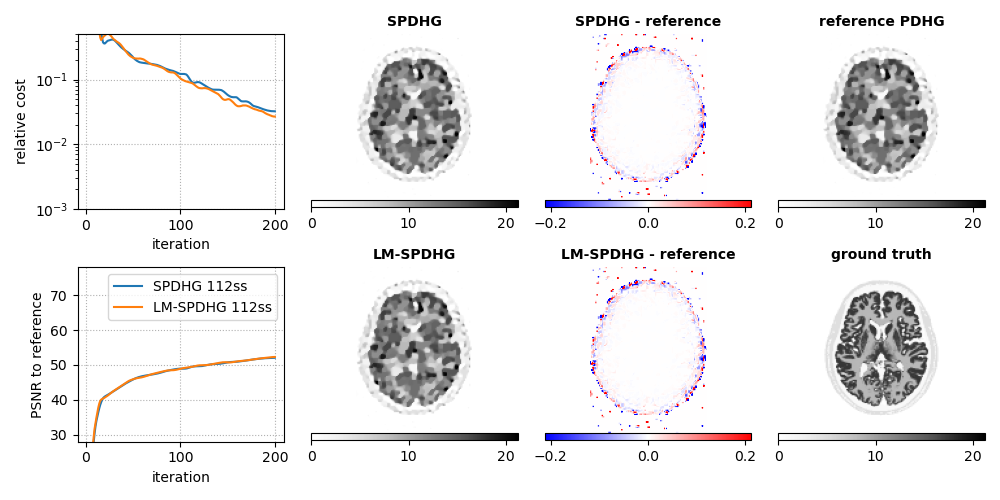
\includegraphics[width=1.0\textwidth]{./figs/brain2d_counts_3.0E+05_seed_1_beta_3.0E-02_prior_TV_niter_ref_20000_fwhm_4.5_4.5_niter_200.png}
    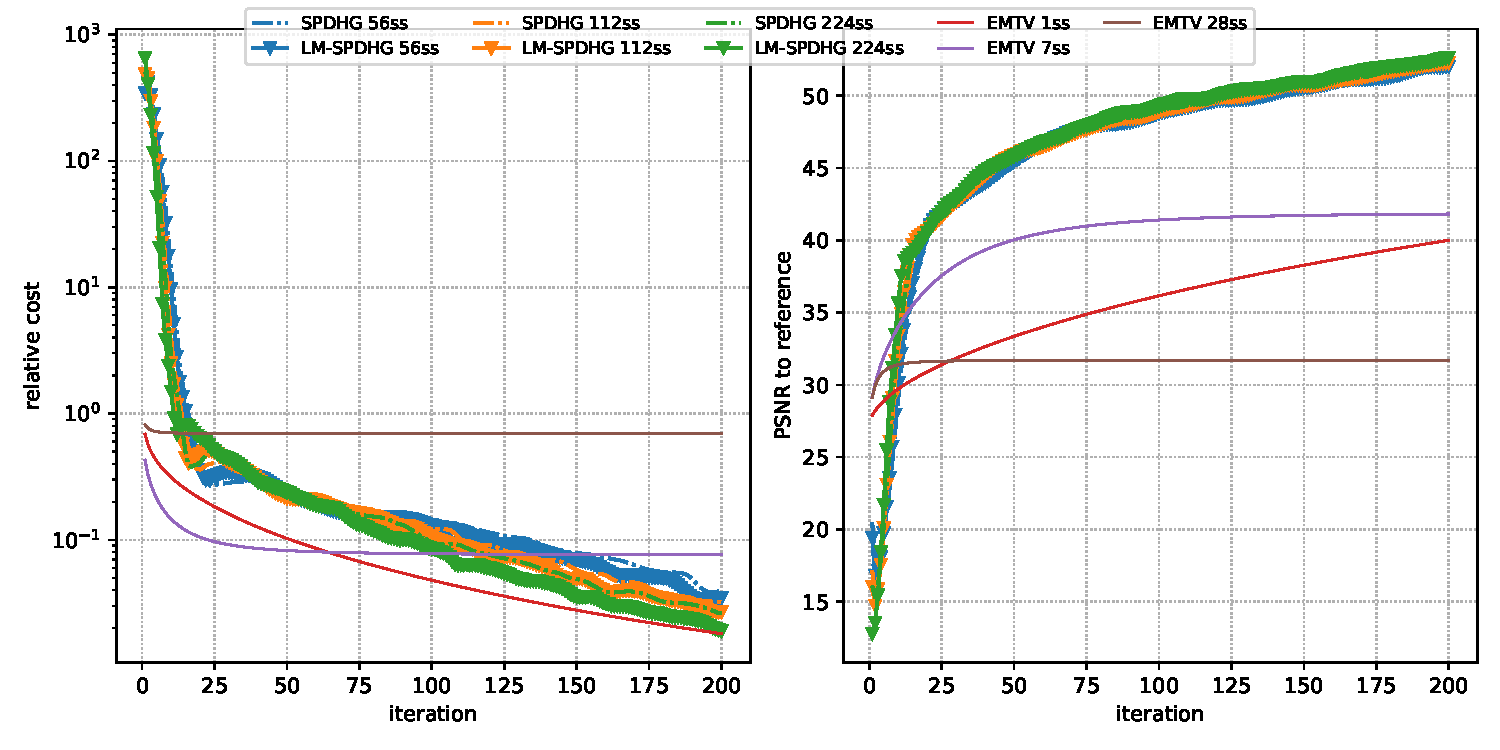
\includegraphics[width=0.8\textwidth]{./figs/brain2d_counts_3.0E+05_seed_1_beta_3.0E-02_prior_TV_niter_ref_20000_fwhm_4.5_4.5_niter_200_metrics.pdf}
  \caption{$3\cdot10^5$ counts, TV, $\beta = 0.03$}
  \label{fig:metrics}
\end{figure*}

\begin{figure*}
  \centering
    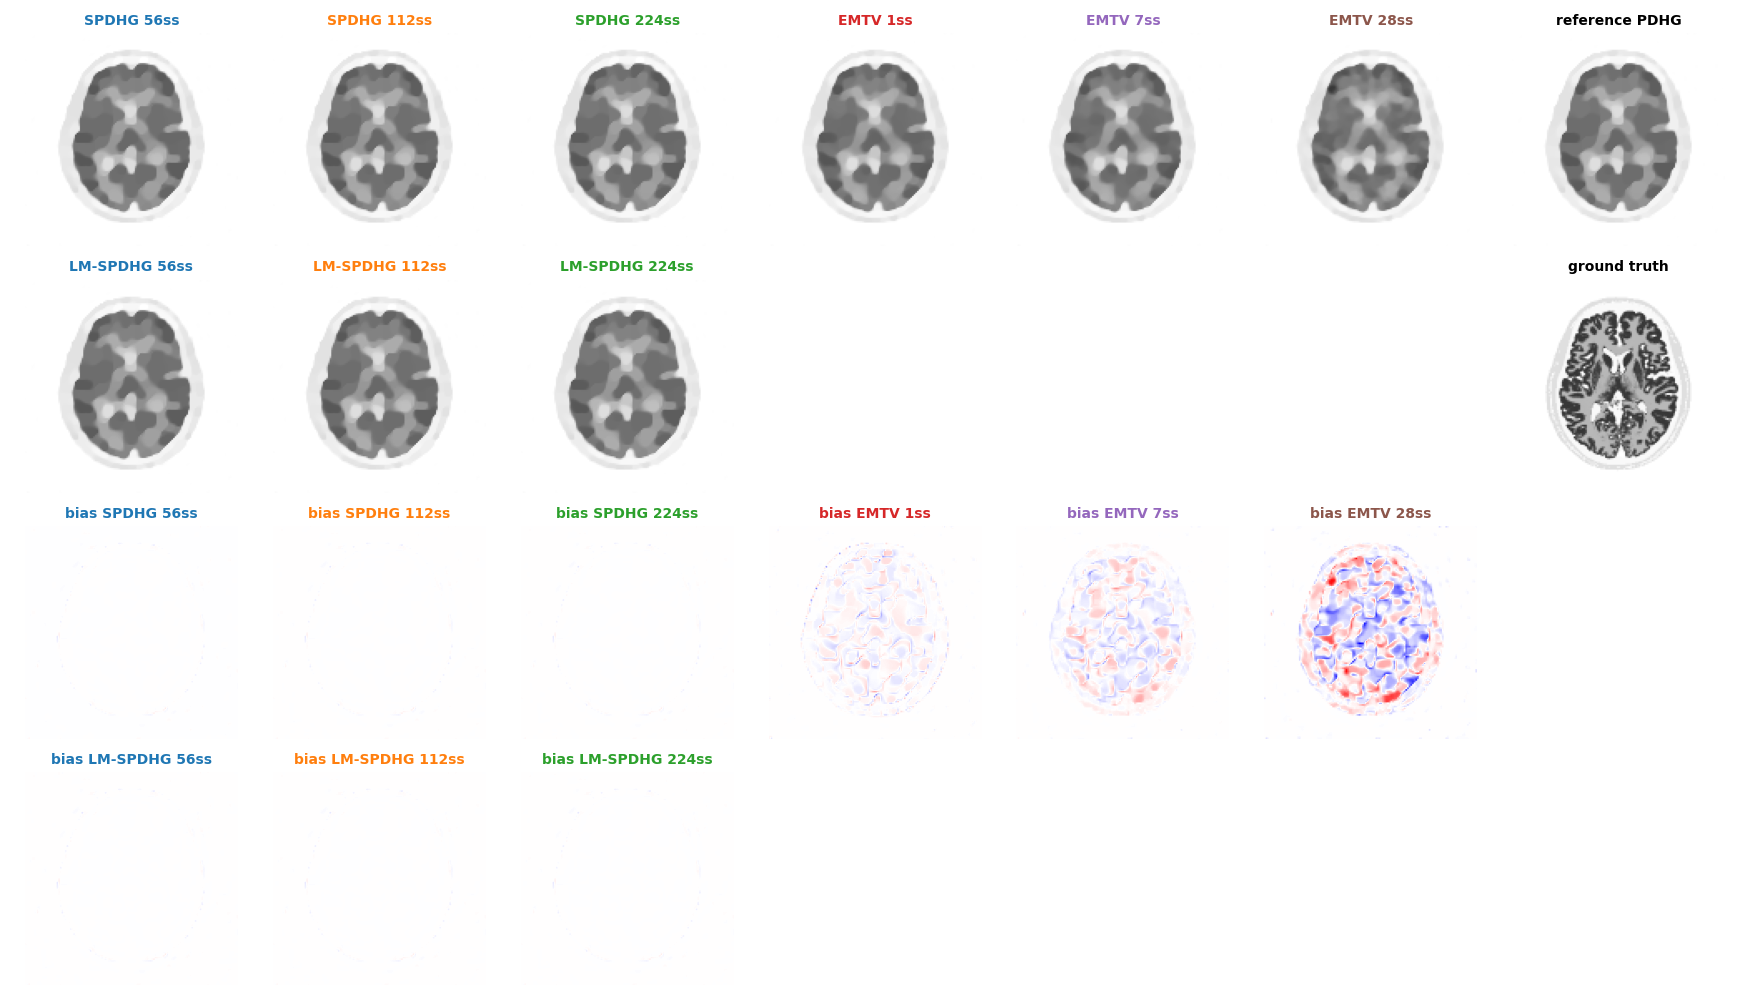
\includegraphics[width=1.0\textwidth]{./figs/brain2d_counts_1.0E+06_seed_1_beta_1.0E-01_prior_TV_niter_ref_20000_fwhm_4.5_4.5_niter_200.png}
    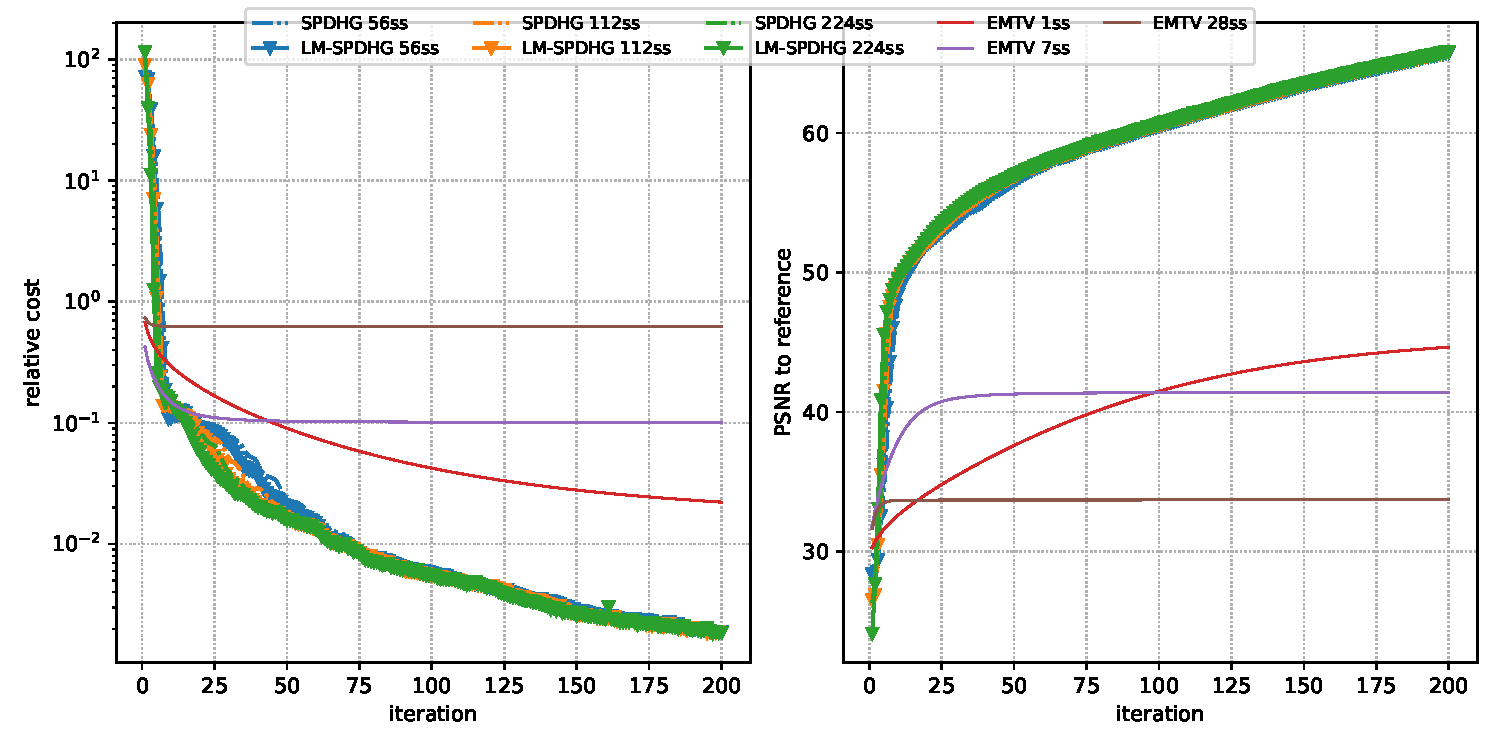
\includegraphics[width=0.8\textwidth]{./figs/brain2d_counts_1.0E+06_seed_1_beta_1.0E-01_prior_TV_niter_ref_20000_fwhm_4.5_4.5_niter_200_metrics.pdf}
  \caption{$1\cdot10^6$ counts, TV, $\beta = 0.1$}
  \label{fig:metrics}
\end{figure*}

\begin{figure*}
  \centering
    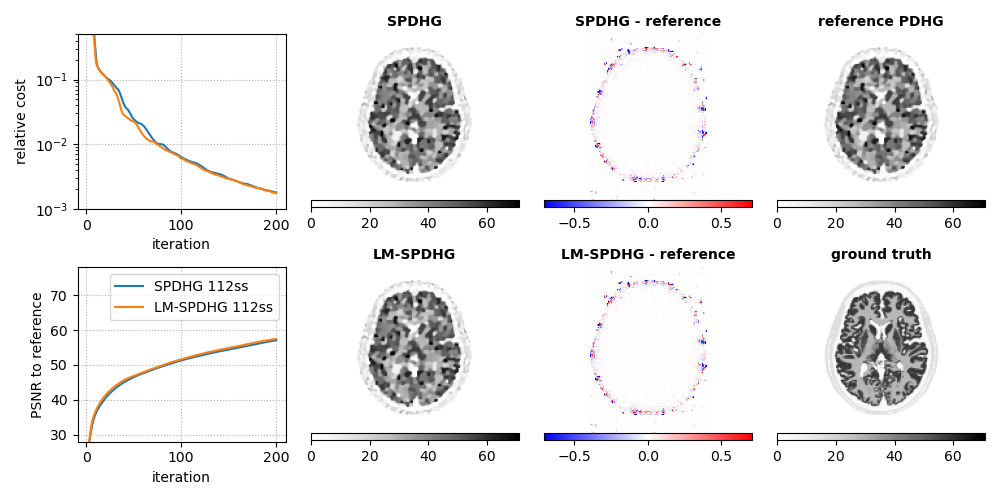
\includegraphics[width=1.0\textwidth]{./figs/brain2d_counts_1.0E+06_seed_1_beta_1.0E-02_prior_TV_niter_ref_20000_fwhm_4.5_4.5_niter_200.png}
    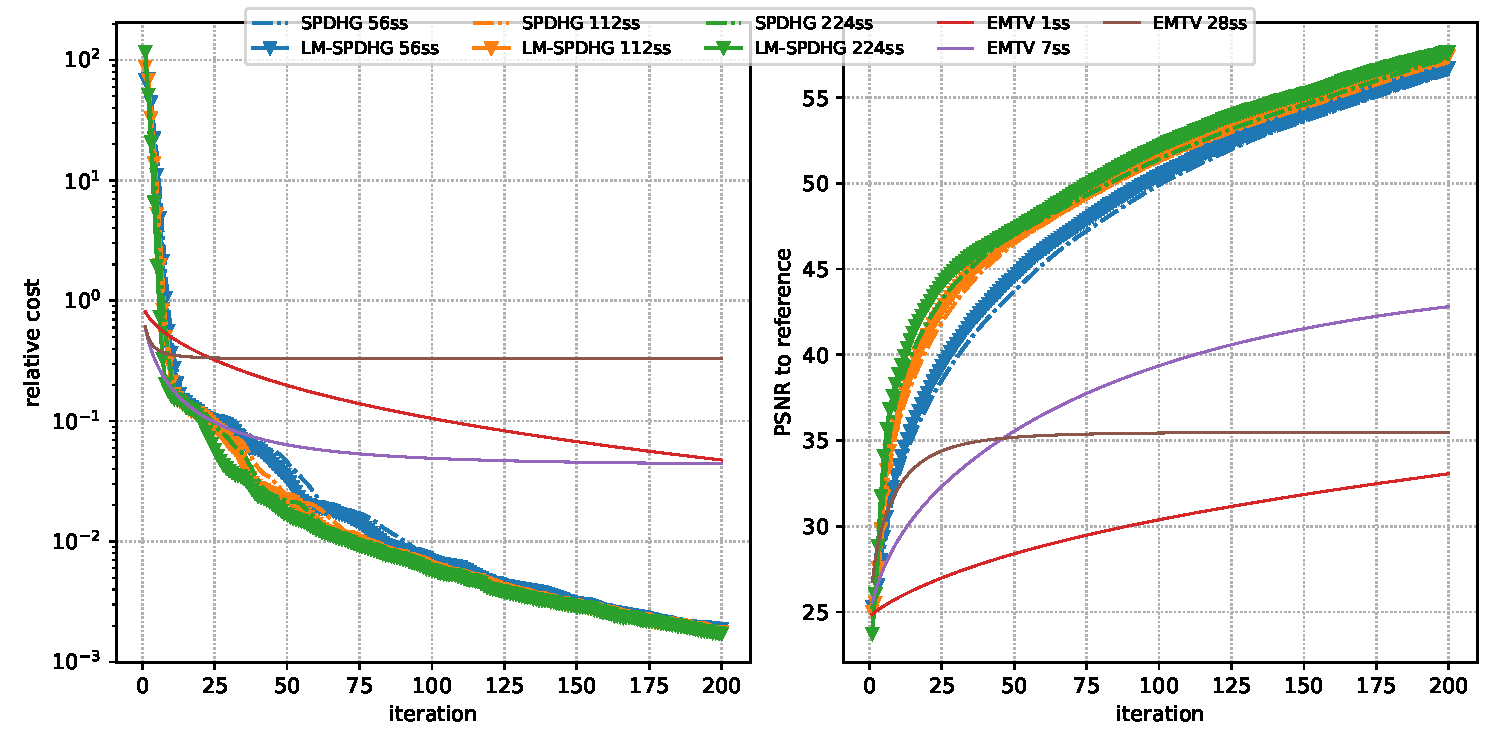
\includegraphics[width=0.8\textwidth]{./figs/brain2d_counts_1.0E+06_seed_1_beta_1.0E-02_prior_TV_niter_ref_20000_fwhm_4.5_4.5_niter_200_metrics.pdf}
  \caption{$1\cdot10^6$ counts, TV, $\beta = 0.01$}
  \label{fig:metrics}
\end{figure*}

\begin{figure*}
  \centering
    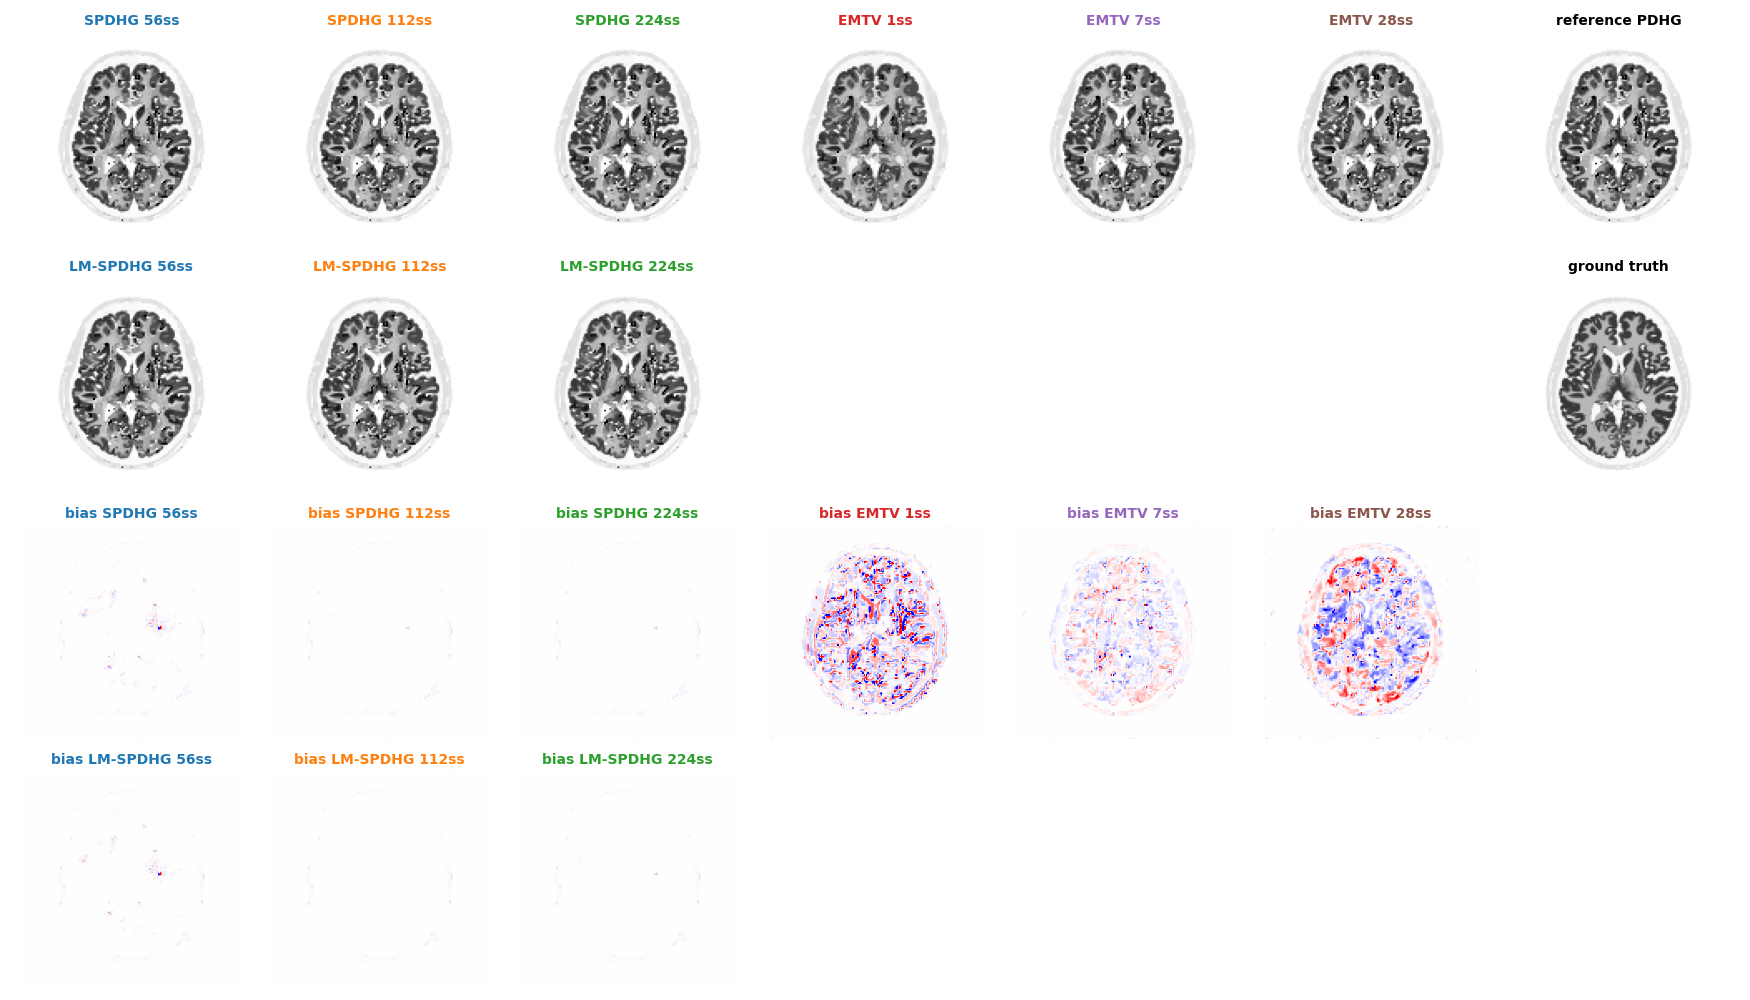
\includegraphics[width=1.0\textwidth]{./figs/brain2d_counts_1.0E+06_seed_1_beta_1.0E-01_prior_DTV_niter_ref_20000_fwhm_4.5_4.5_niter_200.png}
    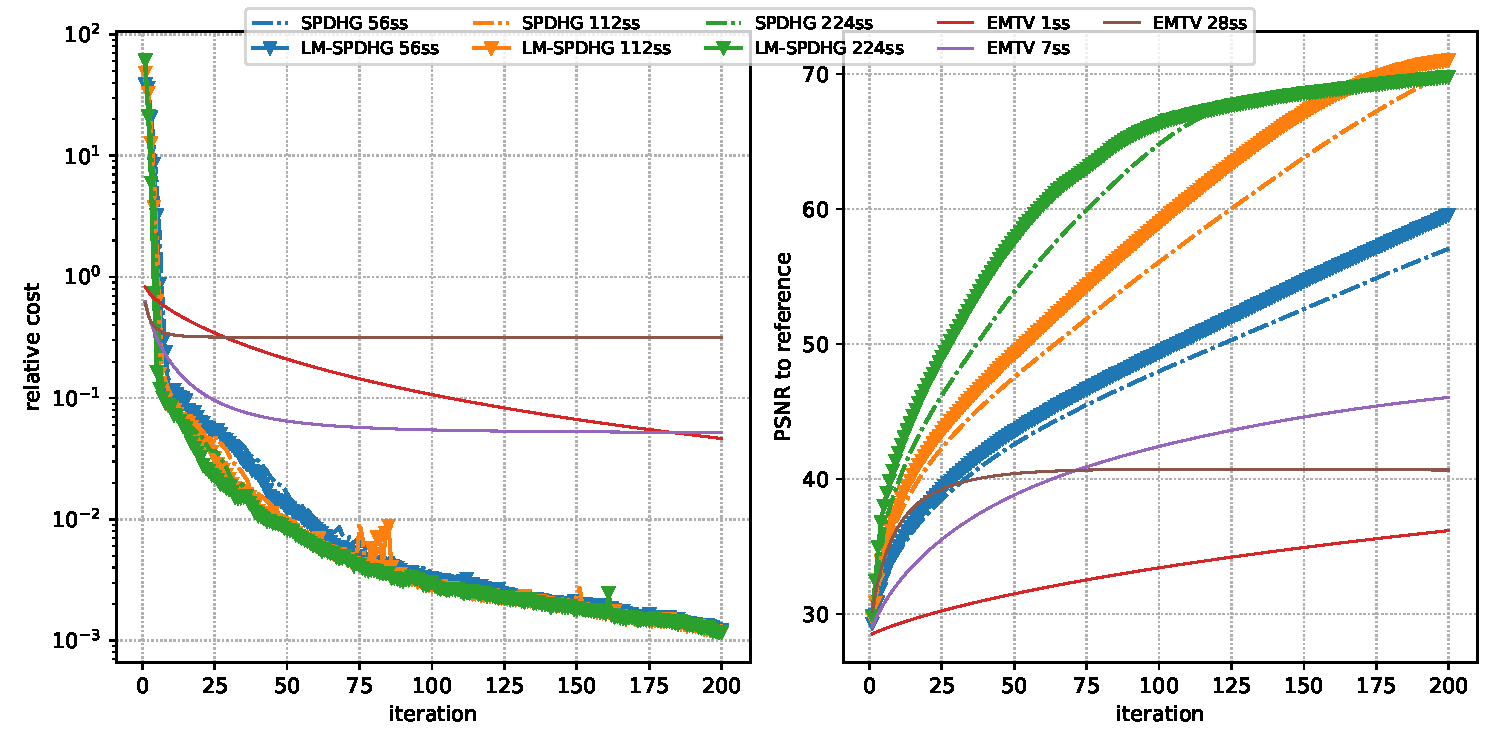
\includegraphics[width=0.8\textwidth]{./figs/brain2d_counts_1.0E+06_seed_1_beta_1.0E-01_prior_DTV_niter_ref_20000_fwhm_4.5_4.5_niter_200_metrics.pdf}
  \caption{$1\cdot10^6$ counts, DTV, $\beta = 0.1$}
  \label{fig:metrics}
\end{figure*}




%-------------------------------------------------------------------------------------------
%\printbibliography

\end{document}
